\section{Digital Signatures using Elliptic Curve Cryptography}

One way to ensure, that a message has not been changed in any way, is to send along the corresponding hash value, which is unique for this message, or more specifically, the odds for a different message to have the same hash value are astronomically low. Note, that this only provides a solution for accidentally modified data. If a man in the middle accomplishes to obtain and alter the to be sent information, it is no further effort to recompute the new hash value as well. However, for our definition of data integrity, this must not be possible. In order to achieve the required level of security, we use asynchronous keys to encrypt the computed hash. By encrypting the hash with the sender's private key and decrypting it with the corresponding public key, we can be certain, that a matching hash value must originate from the owner of the private key, used for the encryption. 
One of the most popular encryption algorithms is RSA. However, nowadays, there are quite a few alternatives to choose from, which offer a variety of advantages compared to RSA. One of which is Elliptic Curve Cryptography. 

\subsection{Curve25519}
This section concentrates on a specific elliptic curve called Curve25519 and its benefits.
Due to this topic's mathematical complexity, the curve will be explained using only the graphical approach.
First of all, an elliptic curve is not an ellipse. The shape of an elliptic curve varies depending on its underlying formula. Fig. \ref{ec1} shows a basic example.
\begin{figure}
\centering
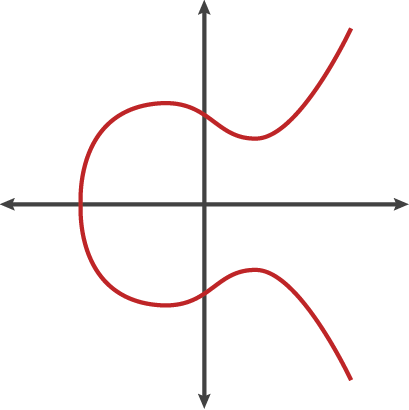
\includegraphics[width=5cm]{Pages/EC/ec.png}
\caption{Example of an elliptic curve \\ (Source: i.stack.imgur.com/ocgjq.png)}
\label{ec1}
\end{figure}

\subsubsection{So how can we encrypt data using a curve?}
As with any other public-private key encryption algorithm, we have to create a random number, only that in our case, this will already be our private key N. In addition, we need a point G on the curve to generate the public key. In order to do so, we have to understand two fairly simple operations, that we can use for points on an elliptic curve.
1. Addition of two points (Fig. \ref{ec2}a): Adding to points A and B to another happens not by simply adding up their x and y coordinates but by the following procedure: By drawing a line through A and B, we intersect the curve at exactly one other point. We reflect this point over the x-axis to get A + B. This is always possible because an elliptic curve is axisymmetric to the x-axis.
2. Addition of a point to itself (Fig. \ref{ec2}b): Adding a point P to itself is very similar to adding up two different points, but instead of the line intersecting three different points, we have a tangent that touches the graph at P and intersects at another point, which again needs to be reflected over the x-axis to get P + P or 2P.
Using these two operations, either doubling a point or adding two points together, we can find any point on the curve that is a multiple of the point we started with. Exactly this resulting point on the graph, which is the product of N * G, will be the public key.

\begin{figure}%
    \centering
    \subfloat[elliptic curve point addition]{{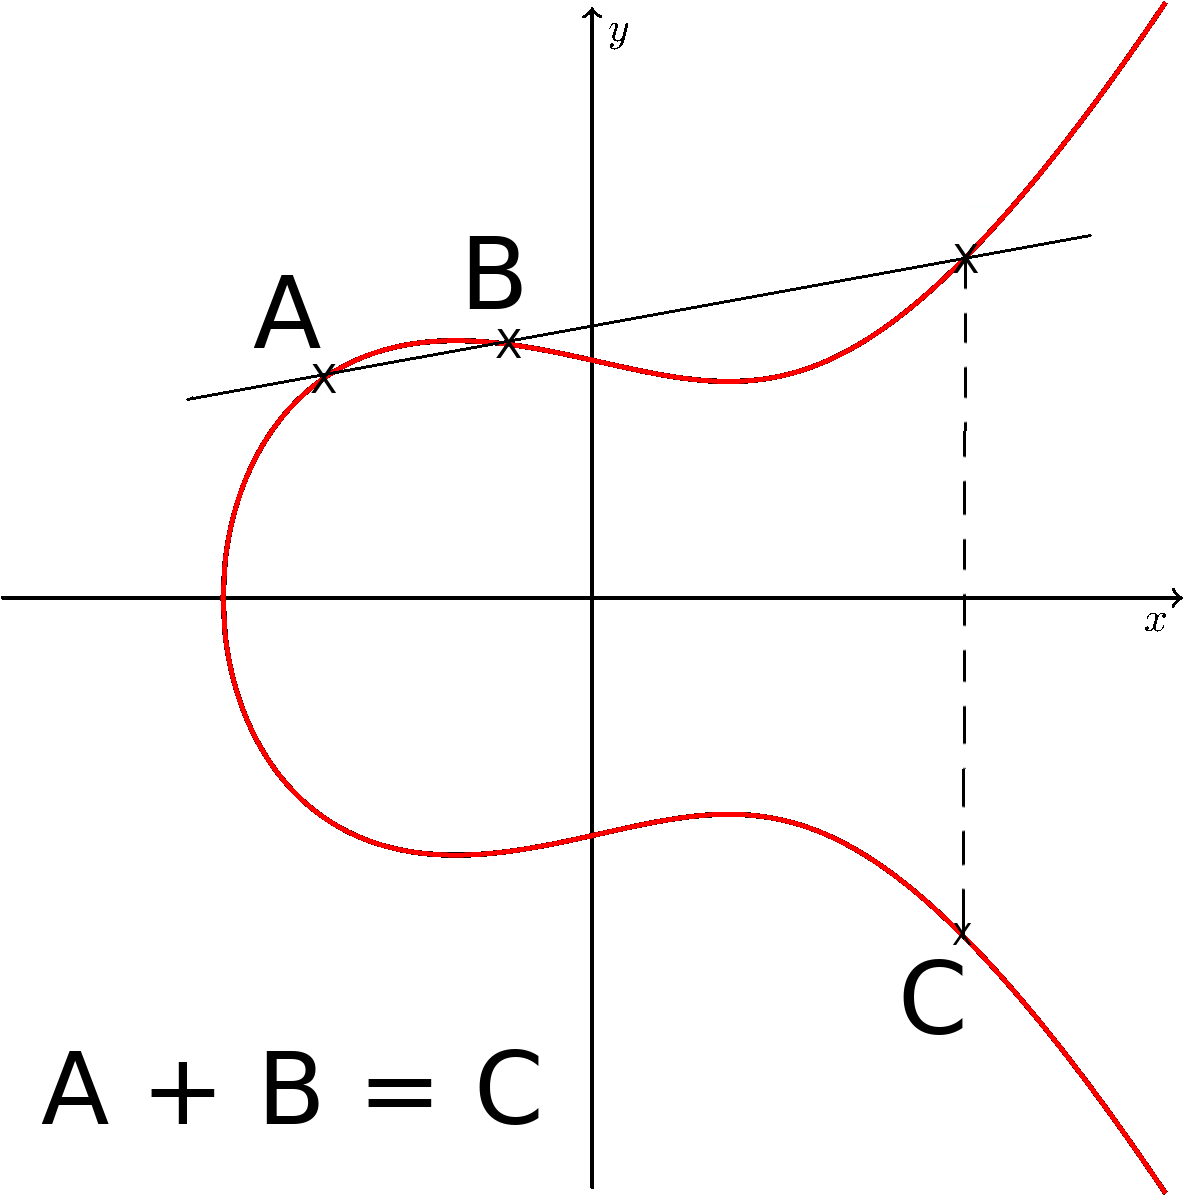
\includegraphics[width=5.5cm]{Pages/EC/ec8.png} }}%
    \qquad
    \subfloat[elliptic curve point multiplication]{{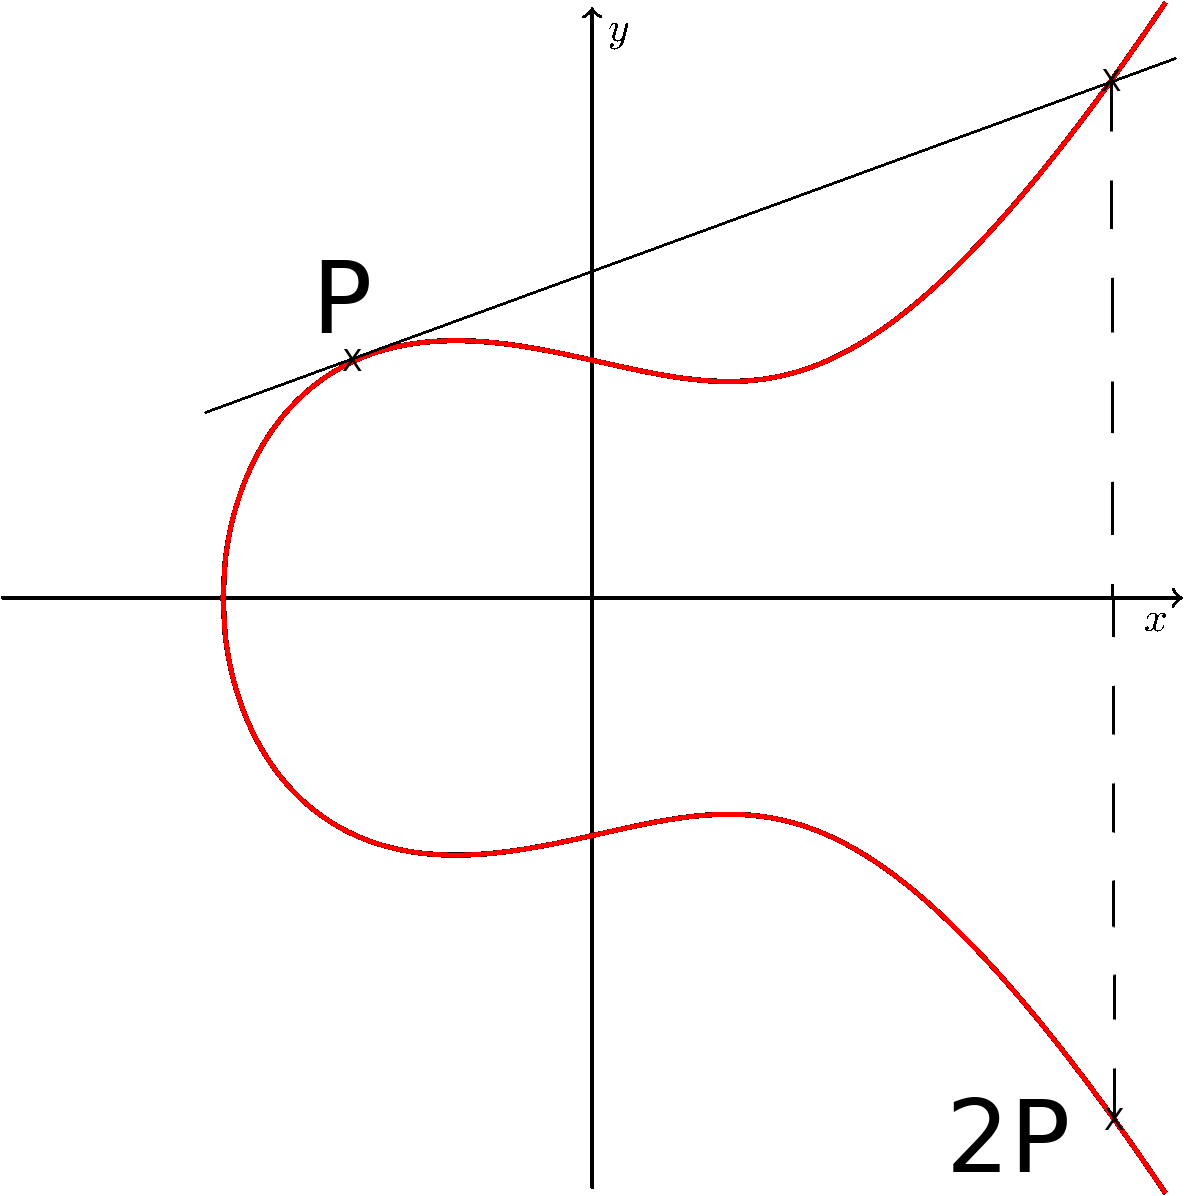
\includegraphics[width=5.5cm]{Pages/EC/ec14.png} }}%
\caption{Operations on an elliptic curve \\ (modifactions of Fig. \ref{ec1})}%
\label{ec2}
\end{figure}

\subsubsection{So why does this provide a secure way to encrypt data?}
In order to crack the encryption, one would have to find the secret number N, which is only possible by checking every multiple of G against the public key and since N is a 256-bit number, this would take many years of computation.
Encryption, on the other hand, is fast, because we do not have to make N multiplications to get to N * G. To clarify, consider the following example:
We choose N to be 1025. In order to compute N * G we then only have to double G ten times to get 1024 * G and finally add this point to G to get 1025 * G, making it a total of 11 operations instead of 1025 and because of the nature of exponential growth, this advantage becomes even more significant, the bigger the private key N gets.

\subsection{Advantages of Curve25519}
\subsubsection{Speed}
The main focus of the original paper about Curve25519 was on its speed. It even broke the current record for the Diffie-Hellman key exchange \cite{ECDH}. For Signatures, it has been shown that a ``quad-core 2.4GHz Intel Westmere (Xeon E5620) CPU can create 109000 signatures per second and verify 71000 signatures'' \cite{Curve25519}. One risk, that needs to be considered when trying to improve the speed of an algorithm, is, that the security could be compromised in the process. As Bernstein, Duif, Lange, Schwabe, Yang \cite{Curve25519} point out, the opposite is the case. Curve25519, in fact, provides additional layers of security like foolproof session keys. One important thing, however, to keep in mind when emphasizing the speed advantages, is, that for larger messages the overall computation time “is dominated by hashing time” \cite{Curve25519}, because while signing time remains constant for increasing message sizes, hashing time grows linearly. 

\subsubsection{Low memory consumption}
For some devices with less memory and small CPUs it can be too much of a computation to use digital signatures, if the size of the public and private keys are too big. Curve25519 uses 32 bytes for private keys and 64 bytes for public keys, although it is even possible to compress the public key to half the size \cite{ECDH}. Compared to the algorithm of RSA, which is recommended by NIST to be using at least 2048 bits or 256 bytes for its keys \cite{NistKeyMan}, this is an immense saving of both memory and necessary computation.

\subsubsection{High security}
Even though Curve25519 uses key sizes of only 32 Byte, it accomplishes to provide a 128-bit security target, meaning it would take $ 2^{128} $ operations to break the encryption \cite{SecLevel}, which is supposed to be secure until “2031 and Beyond” \cite{KeySize}. As mentioned before, RSA uses 2048 bit keys, while only providing $ 2^{112} $ security target. In order to provide the same level of security using RSA, one would have to use 3072 bit key sizes \cite{KeySize}. Note, that this discrepancy gets even bigger as higher security targets are required. For a 128-bit security level, RSA requires twelve times more memory for its keys, than Elliptic Curve Cryptography does. For a 192-bit security level, this factor increases from 12 to more than 20 \cite{SecLevelInc}.

\subsection{Disadvantages of Curve25519}
There are really no obvious negative aspects of Curve25519, since it did not give up any feature of elliptic curves, in order to gain the increase of speed. One thing however, one could argue against not only Curve25519 but elliptic curves in general, is, that this topic's mathematical complexity makes it impossible for an average programmer to understand the algorithm let alone implement it himself. This requires developers to trust on the few people, who completely understand the math behind elliptic curves.

\subsection{Impact on MQTT packet}
For demonstration, this paragraph shows...
\begin{table}[]
\centering
\begin{tabular}{lllllllllllllllll}
45 & 00 & 00 & 8d & 28 & c9 & 40 & 00 &  & 80 & 06 & ec & 47 & c0 & a8 & b2 & 02 \\
c0 & a8 & b2 & 06 & e6 & a4 & 07 & 5b &  & 8b & bf & b9 & 65 & fb & 88 & a4 & e7 \\
50 & 18 & 01 & 00 & 05 & b0 & 00 & 00 &  & 30 & 81 & 23 & 00 & 13 & 2f & 69 & 73 \\
2f & 69 & 74 & 2f & 6f & 66 & 2f & 69 &  & 6e & 74 & 65 & 67 & 72 & 69 & 74 & 79 \\
69 & 6e & 74 & 65 & 67 & 72 & 69 & 74 &  & 79 & 20 & 63 & 61 & 6e & 20 & 62 & 65 \\
20 & 67 & 75 & 61 & 72 & 61 & 6e & 74 &  & 65 & 65 & 64 & 2c & 20 & 69 & 66 & 20 \\
79 & 6f & 75 & 20 & 61 & 72 & 65 & 20 &  & 61 & 62 & 6c & 65 & 20 & 74 & 6f & 20 \\
72 & 65 & 63 & 61 & 6c & 63 & 75 & 6c &  & 61 & 74 & 65 & 20 & 74 & 68 & 69 & 73 \\
20 & 70 & 61 & 72 & 74 & 3a & 30 & 45 &  & 02 & 21 & 00 & de & b1 & 60 & fd & 41 \\
53 & 16 & 1a & e0 & 9a & a7 & 0e & bc &  & 20 & 09 & 70 & 46 & 78 & 71 & f7 & 5e \\
ca & 9f & fa & 98 & 33 & 8f & e1 & 6d &  & b2 & b0 & dc & 02 & 20 & 51 & 00 & b4 \\
6f & fe & d7 & 9d & 25 & 16 & 6f & 7a &  & 94 & 0f & 39 & f6 & 4f & 18 & 19 & 75 \\
3c & f7 & 71 & 04 & 09 & f1 & 47 & 1b &  & 3f & 04 & 6c & 31 & 4a &    &    &    \\   
\end{tabular}
\caption{Write here!}
\label{tab:ecc-table}
\end{table}
